\documentclass[11pt, a4paper]{article}

\usepackage{style}

\author{Vladislav Mlejnecký}

\title{%
  Číslicové zpracování signálů\\
  \large Úloha číslo 5.\\
  Přenosová funkce LTI, kmitočtová charakteristika, nástroje Matlab}

\begin{document}

    \maketitle
    
    \section{Zadání}
    
    \begin{enumerate} 
        \item
        Ověřte, jak se projeví na přenosové funkci číslicové soustavy:
        \begin{enumerate}[label=(\alph*)]
            \item
            FIR a jedna reálná nula přenosu
            \item
            IIR a jeden reálný pól přenosu
            \item
            FIR a jeden pár komplexně sdružených nul
            \item
            IIR a jeden pár komplexně sdružených pólů
            \item
            IIR a jeden pár komplexně sdružených pólů + jeden pár komplexně sdružených nul
        \end{enumerate}
    \end{enumerate}
    
    \section{Výsledné grafy}
    
        \begin{figure}[H]
            \centering
            \begin{minipage}{.5\textwidth}
                \centering
                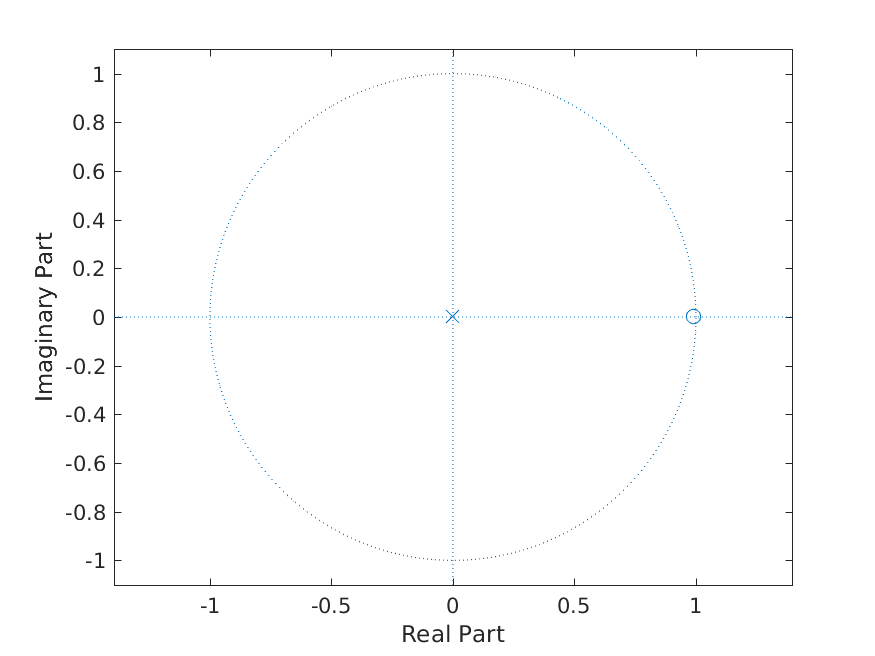
\includegraphics[width=.9\textwidth]{matlab/a1.png}
            \end{minipage}%
            \begin{minipage}{.5\textwidth}
                \centering
                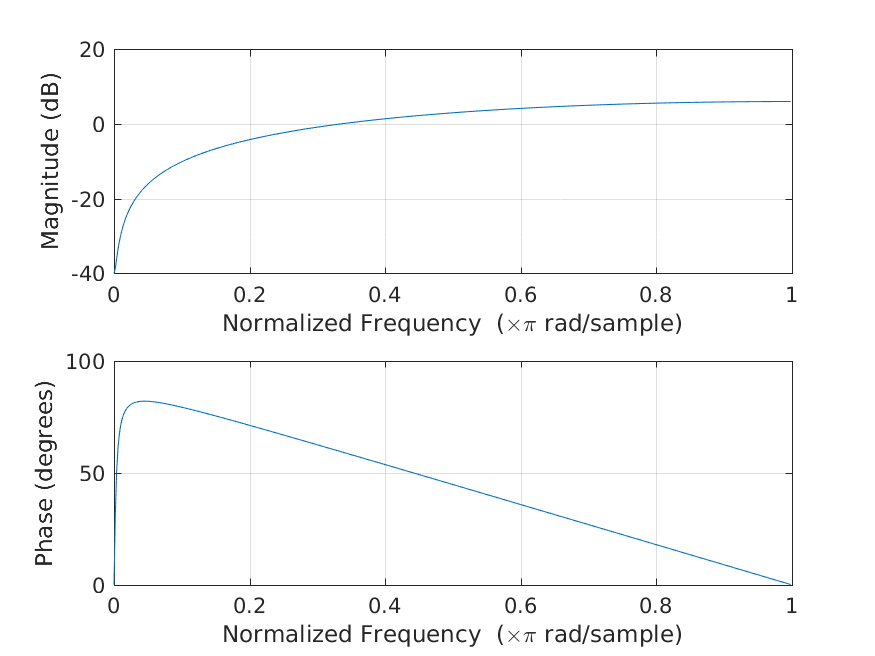
\includegraphics[width=.9\textwidth]{matlab/a2.png}
            \end{minipage}
            \caption{Situace dle bodu zadání A}
            \label{fig:1}
        \end{figure}

        \begin{figure}[H]
            \centering
            \begin{minipage}{.5\textwidth}
                \centering
                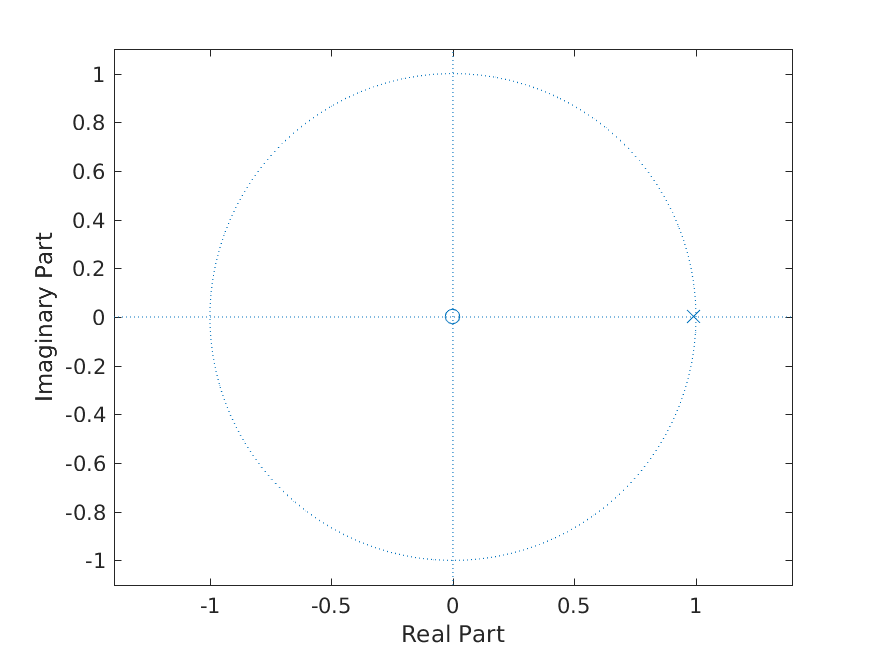
\includegraphics[width=.9\textwidth]{matlab/b1.png}
            \end{minipage}%
            \begin{minipage}{.5\textwidth}
                \centering
                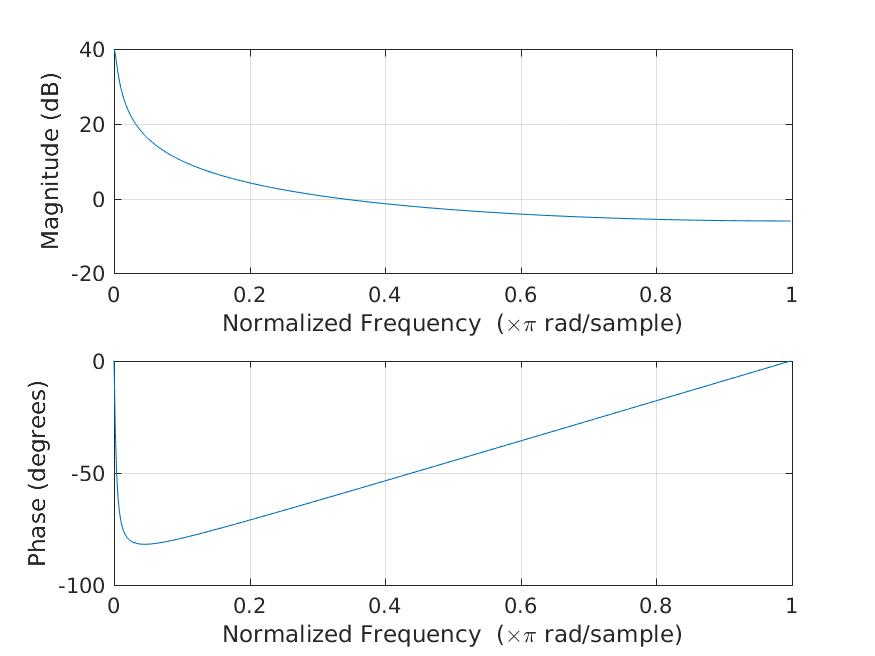
\includegraphics[width=.9\textwidth]{matlab/b2.png}
            \end{minipage}
            \caption{Situace dle bodu zadání B}
            \label{fig:2}
        \end{figure}

        \begin{figure}[H]
            \centering
            \begin{minipage}{.5\textwidth}
                \centering
                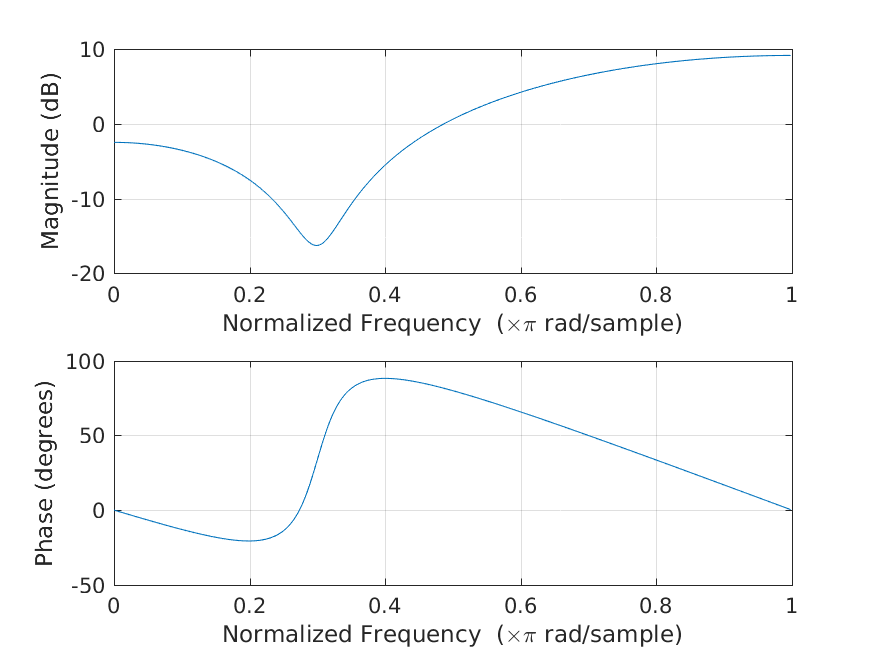
\includegraphics[width=.9\textwidth]{matlab/c1.png}
            \end{minipage}%
            \begin{minipage}{.5\textwidth}
                \centering
                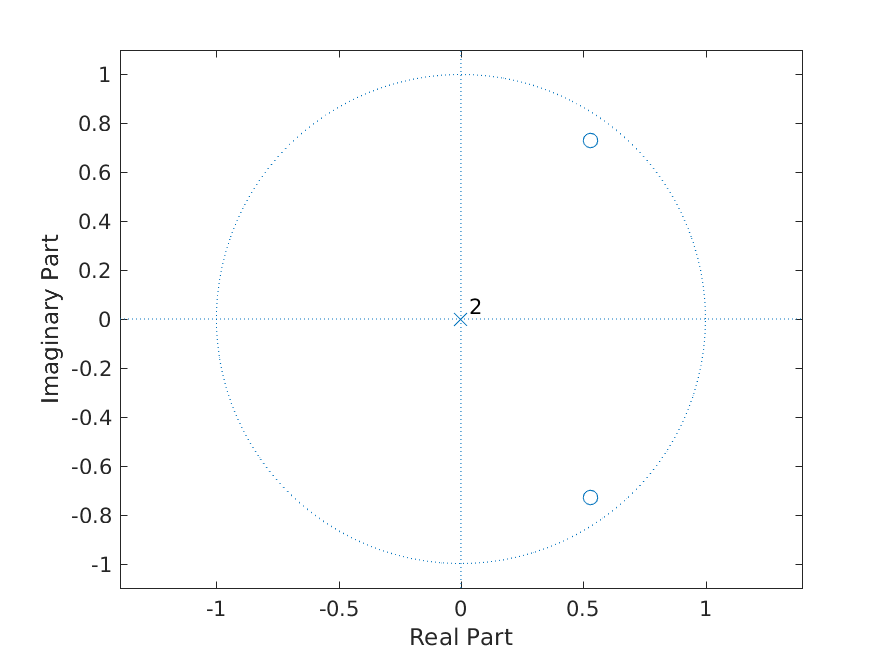
\includegraphics[width=.9\textwidth]{matlab/c2.png}
            \end{minipage}
            \caption{Situace dle bodu zadání C}
            \label{fig:3}
        \end{figure}

        \begin{figure}[H]
            \centering
            \begin{minipage}{.5\textwidth}
                \centering
                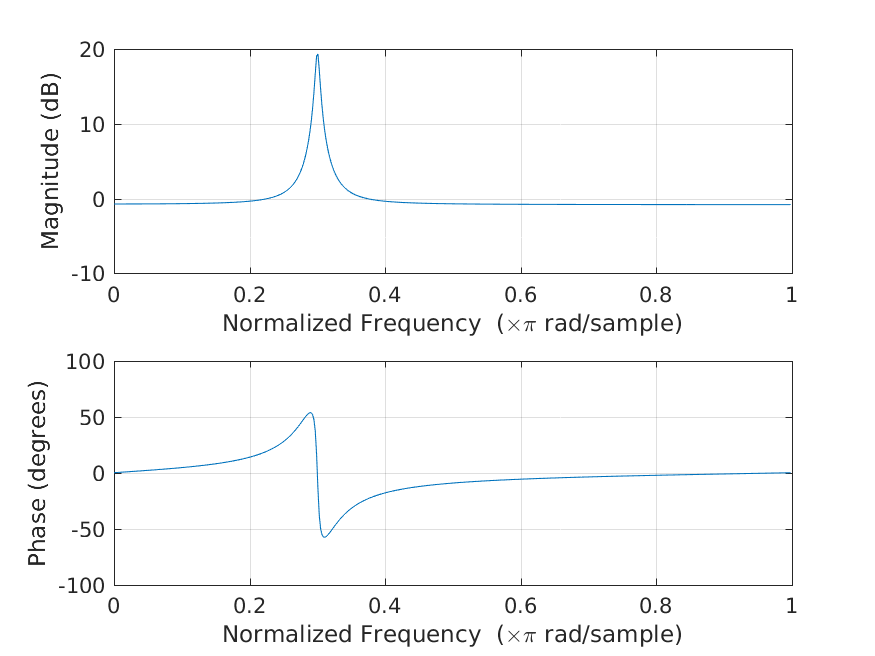
\includegraphics[width=.9\textwidth]{matlab/d1.png}
            \end{minipage}%
            \begin{minipage}{.5\textwidth}
                \centering
                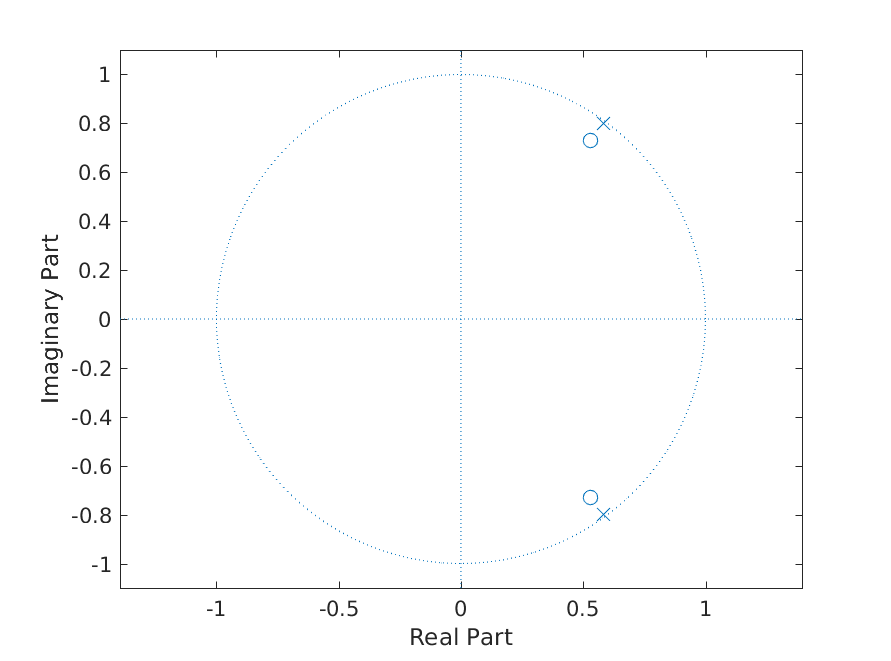
\includegraphics[width=.9\textwidth]{matlab/d2.png}
            \end{minipage}
            \caption{Situace dle bodu zadání D}
            \label{fig:4}
        \end{figure}

        \begin{figure}[H]
            \centering
            \begin{minipage}{.5\textwidth}
                \centering
                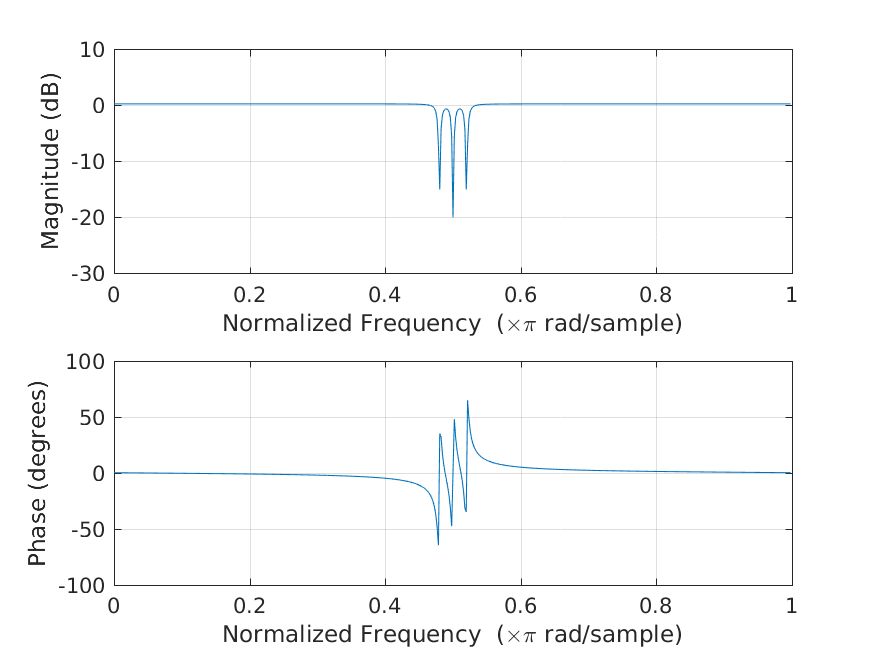
\includegraphics[width=.9\textwidth]{matlab/e1.png}
            \end{minipage}%
            \begin{minipage}{.5\textwidth}
                \centering
                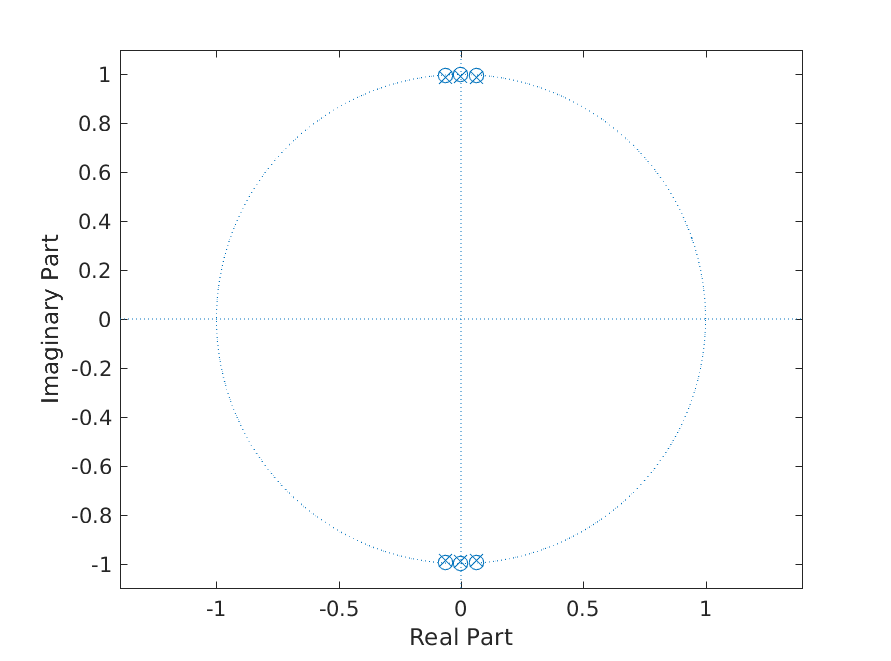
\includegraphics[width=.9\textwidth]{matlab/e2.png}
            \end{minipage}
            \caption{Situace dle bodu zadání E}
            \label{fig:5}
        \end{figure}

    \section{Výpis zdrojového kódu}
    
\begin{lstlisting}[language=matlab, frame=single]    
%a
z1=0.99*exp(1j*pi*0);
a=[1 0];
b=[1 -z1];

h1 = figure();
zplane(b,a);
h2 = figure();
freqz(b,a);

saveas(h1, 'a1.png');
saveas(h2, 'a2.png');

%b
z1=0.99*exp(1j*pi*0);
b=[1 0];
a=[1 -z1];

h3 = figure();
zplane(b,a);
h4 = figure();
freqz(b,a);

saveas(h3, 'b1.png');
saveas(h4, 'b2.png');

%c
z1=0.9*exp(1j*pi*0.3);
z2=conj(z1);
a=[1 0 0];
b=[1 -(z1+z2) z1*z2];

h5 = figure();
freqz(b,a);
h6 = figure();
zplane(b,a);

saveas(h5, 'c1.png');
saveas(h6, 'c2.png');

%d
p1=0.99*exp(1j*pi*0.3); p2=conj(p1);
n1=0.9*exp(1j*pi*0.3); n2=conj(n1);
a=[1 -(p1+p2) p1*p2];
b=[1 -(n1+n2) n1*n2];

h7 = figure();
freqz(b,a);
h8 = figure();
zplane(b,a);

saveas(h7, 'd1.png');
saveas(h8, 'd2.png');

%e
mn=0.999; mp=0.99;
f1=0.48; f2=0.5; f3=0.52;
p1=mp*exp(1j*pi*f1); p2=conj(p1);
p3=mp*exp(1j*pi*f2); p4=conj(p3);
p5=mp*exp(1j*pi*f3); p6=conj(p5);

n1=mn*exp(1j*pi*f1); n2=conj(n1);
n3=mn*exp(1j*pi*f2); n4=conj(n3);
n5=mn*exp(1j*pi*f3); n6=conj(n5);

a=[1 -(p1+p2) p1*p2];
b=[1 -(n1+n2) n1*n2];

a=conv(a,[1 -(p3+p4) p3*p4]);
a=conv(a,[1 -(p5+p6) p5*p6]);
b=conv(b,[1 -(n3+n4) n3*n4]);
b=conv(b,[1 -(n5+n6) n5*n6]);

h9 = figure();
freqz(b,a);
h10 = figure();
zplane(b,a);

saveas(h9, 'e1.png');
saveas(h10, 'e2.png');
\end{lstlisting}

\end{document}
